\documentclass[12pt,a4paper]{article}
\usepackage[legalpaper, portrait, margin=3cm]{geometry}
\usepackage{fancyhdr}
\usepackage{amsmath}
\usepackage{amssymb}
\usepackage{graphicx}
\usepackage{blindtext}
\usepackage{hyperref}
\usepackage{indentfirst}
\usepackage{float}
\usepackage{biblatex}
\usepackage[Symbol]{upgreek}

\graphicspath{ {./} }
\hypersetup{
  colorlinks=true,
  linkcolor=blue,
  filecolor=magenta,
  urlcolor=blue,
  citecolor=blue,
  pdftitle={Relatório ASA - Projeto 2 - 2022/2023},
  pdfpagemode=FullScreen,
}
\addbibresource{./bibliography.bib}

\pagestyle{fancy}
\fancyhf{}
\rhead{Grupo \textbf{al013}}
\lhead{Relatório Projeto 2 ASA 2022/2023 LEIC-A}
\cfoot{Gonçalo Sampaio Bárias (103124)}

\renewcommand{\footrulewidth}{0.2pt}

\renewcommand{\labelitemii}{$\circ$}
\renewcommand{\labelitemiii}{$\diamond$}

\begin{document}
  \section{Descrição do Problema e da Solução}

  \section{Análise Teórica}

  \section{Avaliação Experimental dos Resultados}

  Foram gerados vários grafos com um número de arestas entre 10 e 10 000 000, todos diferentes entre si. Para cada ordem de grandeza de arestas foram gerados pelo menos 100 grafos, tendo um total de 541 grafos.
  O programa foi executado, pelo menos 100 vezes para cada grafo, recorrendo ao programa de \textit{benchmarking} \href{https://github.com/sharkdp/hyperfine}{\textit{hyperfine}}.

  \begin{figure}[H]
    \centering
    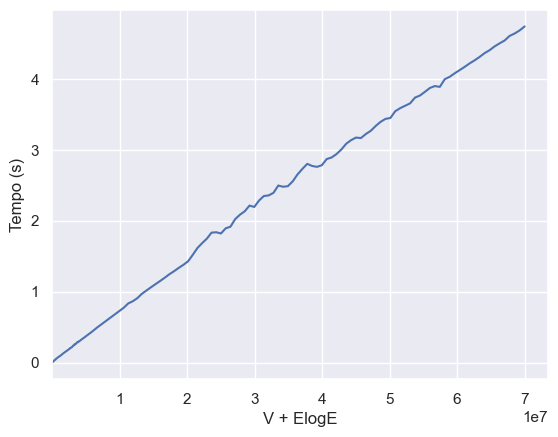
\includegraphics[width=4in]{report.png}
    \caption{Complexidade temporal do problema proposto}
    \label{fig:graphic}
  \end{figure}

  O gráfico apresentado tem o número de arestas no eixo dos $xx$ com uma escala $E \log E$ e o tempo em segundos no eixo dos $yy$.
  Os dados revelam uma tendência linear, comprovando que a complexidade temporal do problema é, num caso geral, $O(E\log E)$, tal como concluído na análise teórica.

  \printbibliography[title={Referência}]

\end{document}
Footer
